%!TEX root = ../thesis.tex

%-----------------------------------------------------------------------------%
% DOCUMENT
%-----------------------------------------------------------------------------%
\documentclass[
    pdftex,
    % Print only one side of a paper, alternate: twoside
    oneside,
    % Font size (recommended by DHBW)
    12pt,
    % Don't indent space for each paragraph
    parskip=half,
    % Needed to add indices to tableofcontents
    listof=totoc,
    bibliography=totoc,
    % Change the header and footer height
    headheight=26pt,
    footheight=16pt,
    %
    headinclude=false,
    footinclude=false,
    % Add a seperation line for the header
    headsepline,
    % Some modifications for the pdf document
    % Needed the `geometry` package loaded and margin set to work correctly.
    DIV=calc,
    BCOR=8mm,
    appendixprefix
]{scrartcl}

%-----------------------------------------------------------------------------%
% ENCODING
%-----------------------------------------------------------------------------%
% Support other language encodings, e.g. 'ä', 'ö', 'ü'. Include this packages 
% in every latex document.
\usepackage[utf8]{inputenc}
\usepackage[T1]{fontenc}

%-----------------------------------------------------------------------------%
% PACKAGES
%-----------------------------------------------------------------------------%

% Use the following babel packages, set last as default.
% Add other languages if necessary.
\usepackage[english, ngerman]{babel}

% Use prettier font.
% Other fonts: palatino, goudysans, lmodern, libertine
\usepackage{lmodern}

% Change the default margin of the document. You can change the values for your
% beheviour
\usepackage[foot=1.0cm, margin=2.5cm]{geometry}

% Include figures.
\usepackage{graphicx}

% Needed to place images at code position
\usepackage{float}

% Use strings and make string operations, such as \IfStrEq available.
\usepackage{xstring}

% Use substring operations.
% Needed to know how many authors writing on the thesis.
\usepackage{substr}

% Enable `\rgb` command to define custom colors.
% Needed by some modules, e.g. for listings.
\usepackage{xcolor}
%!TEX root = ../thesis.tex

%-----------------------------------------------------------------------------%
% COLORS
%-----------------------------------------------------------------------------%

\definecolor{background}{rgb}{0.94, 0.94, 0.94}
\definecolor{codegray}{rgb}{0.5,0.5,0.5}

% Enables doublespacing. This improves the layout for the cover a lot.
% It is recommended to use this package, so it is in the base module.
\usepackage[onehalfspacing]{setspace}

% Use \cite, \parencite, for citations.
\usepackage{csquotes}

% The next three packages are useful to enable hyperrefs and bookmarking for pdf
% documents.
% Don't delete any of these packages and don't rearrange them. This could cause
% unexpected issues.
\usepackage{pdfpages}

% Commands for if statements.
\usepackage{ifthen}

% Enable the ability to use \pagestyle{fancy} with custom headers.
% This package is optional but is installed in most LaTeX distribution by
% default.
\usepackage{fancyhdr}

\usepackage{enumerate}

%-----------------------------------------------------------------------------%
% COMMANDS
%-----------------------------------------------------------------------------%
%!TEX root = ../thesis.tex

%-----------------------------------------------------------------------------%
% COMMANDS
%-----------------------------------------------------------------------------%

% Document language
\newcommand{\setDocumentLanguage}[1]{\def\documentLanguage{#1}}

% Document type
\newcommand{\setDocumentType}[1]{\def\documentType{#1}}

% Title
\newcommand{\setDocumentTitle}[1]{\def\documentTitle{#1}}

% Author
\newcommand{\setDocumentAuthor}[1]{\def\documentAuthor{#1}}

% Matriculation number
\newcommand{\setMatriculationNumber}[1]{\def\matriculationNumber{#1}}

% Course name
\newcommand{\setCourse}[1]{\def\course{#1}}

% Location of the university
\newcommand{\setLocationUniversity}[1]{\def\locationUniversity{#1}}

% Release date
\newcommand{\setReleaseDate}[1]{\def\releaseDate{#1}}

% Release location
\newcommand{\setReleaseLocation}[1]{\def\releaseLocation{#1}}

% Period
\newcommand{\setDocumentPeriod}[1]{\def\documentPeriod{#1}}

% Department
\newcommand{\setDepartment}[1]{\def\department{#1}}

% Lecture
\newcommand{\setLecture}[1]{\def\lecture{#1}}

% Degree
\newcommand{\setDegree}[1]{\def\degree{#1}}

% Name of the tutor
\newcommand{\setTutor}[1]{\def\tutor{#1}}

% Name of the evaluator
\newcommand{\setEvaluator}[1]{\def\evaluator{#1}}

% Company name
\newcommand{\setCompanyName}[1]{\def\companyName{#1}}

% Company location
\newcommand{\setCompanyLocation}[1]{\def\companyLocation{#1}}

% Restriction
\newcommand{\restrictDocument}[1]{\def\restricted{#1}}

% Electronic
\newcommand{\hasElectronicVersion}[1]{\def\electronicVersion{#1}}

% Company logo
\newcommand{\showCompanyLogo}[1]{\def\companyLogo{#1}}

% DHBW logo
\newcommand{\showDHBWLogo}[1]{\def\dhbwLogo{#1}}

% Point out code
\newcommand{\setEmphraseCode}[1]{\def\emphraseCode{#1}}

% Quote style
\newcommand{\setQuoteStyle}[1]{\def\quoteStyle{#1}}

%-----------------------------------------------------------------------------%

% Check document type.
\newcommand{\IfDocType}[3]{%
    \IfStrEq{\documentType}{#1}{#2}{#3}%
}%

% Check if string is empty.
\newcommand{\IfStrIsEmpty}[3]{%
    \IfStrEq{#1}{}{#2}{#3}%
}%

% Write text in code style.
\newcommand{\code}[1]{%
    \IfStrEq{\emphraseCode}{yes}{%
        \colorbox{background}{\texttt{#1}}%
    }{% else
        \texttt{#1}%
    }
}%

%-----------------------------------------------------------------------------%

% % Generate appendix table of contents
% % Working solution without extra packages (KOMA) from:
% % https://tex.stackexchange.com/questions/260445/separate-table-of-contents-for-appendix
% \DeclareNewTOC[%
%     owner=\jobname,
%     listname={\appendixname}, % title of the appendix toc
% ]{atoc}

% \makeatletter
% \newcommand*\appendixwithtoc{%
%     \cleardoublepage%
%     \appendix%
%     \addcontentsline{toc}{chapter}{\appendixname}%
%     \renewcommand*{\ext@toc}{atoc}%
%     \scr@ifundefinedorrelax{hypersetup}{}{\hypersetup{bookmarkstype=atoc}}%
%     \listofatocs
% }
% \makeatother

%-----------------------------------------------------------------------------%

%-----------------------------------------------------------------------------%
% SETTINGS
%-----------------------------------------------------------------------------%
%!TEX root = ../document.tex

%-----------------------------------------------------------------------------%
% Settings marked with * are required.
%-----------------------------------------------------------------------------%

% Document language*
% If the language is not supported yet, you can define your own language file or
% use the default (en_US).
\setDocumentLanguage{de_DE}

% Document type*
% Available types:
% t1000    - Template for T3_1000 (project thesis, evaluator from company)
% t2000    - Template for T3_2000 (project thesis, evaluator from university)
% t3000    - Template for T3_3000 (project thesis, evaulator from company)
% seminar  - Template for T3_3300 (seminar thesis, evaluator from university)
% bachelor - Template for bachelor thesis (evaluator from company and
%            university)
\setDocumentType{Tutorial}

% Title*
% The title should not be longer than two lines.
\setDocumentTitle{Particle Swarm Algorithmus}

% Author*
\setDocumentAuthor{5703004, 1716504}

% Matriculation number*
% Usually a seven-digit number, e.g. 5703134
\setMatriculationNumber{5703004, 1716504}

% Course name*
% Find in on your student ID, e.g. MOS-TINF19B
\setCourse{MOS-TINF19B}

% Location of the university*
\setLocationUniversity{Mosbach}

% Release date*
\setReleaseDate{\today}

% Release location*
\setReleaseLocation{Mosbach}

% Period*
% The duration the thesis was written through.
\setDocumentPeriod{}

% Department*
% e.g. Angewandte Informatik
\setDepartment{Angewandte Informatik}

% Lecture
% Optional, if this thesis was written for a specific lecture.
\setLecture{Advanced Software Engineering}

% Degree (required if \documentType{bachelor})
\setDegree{Bachelor of Science}

% Name of the tutor*
\setTutor{Prof. Dr. Carsten Müller}

% Name of the evaluator (required if \documentType{bachelor})
\setEvaluator{}

% Company name
% Leave empty if not required. Only in combination with \setCompanyLocation.
\setCompanyName{}

% Company location
% Leave empty if not required. Only in combination with \setCompanyName.
\setCompanyLocation{}

% Restriction
% Is this document restricted to the public? Set `yes` if so.
\restrictDocument{no}

% Electronic
% Has this document an electronic version? Set `yes` if so.
\hasElectronicVersion{no}

%-----------------------------------------------------------------------------%
% DHBW logo
% Show the DHBW logo on the titlepage? Set `yes` if so.
%
% If the DHBW logo is not rendered correctly, you can change the size inside of
% the cover module in `modules/cover.tex`
\showDHBWLogo{no}

% Company logo
% Show the company logo on the titlepage? Set `yes` if so.
%
% If the company logo is not rendered correctly, you can change the size inside
% of the cover module in `modules/cover.tex`
\showCompanyLogo{no}

% Emphrase code
% Set `yes` if inline \code should be emphrased with gray background.
\setEmphraseCode{yes}

% Quote style
% Set the style of the quotes.
%
% Available types:
% harvard - e.g. (autor year, p.10)
% default - e.g. [1, p.10]
%
% If no style is set, the template will use the default template.
\setQuoteStyle{harvard}

%-----------------------------------------------------------------------------%
% LANGUAGE
%-----------------------------------------------------------------------------%
% Load the language file, if not exists, load default.
\edef\BaseFile{res/i18n/\documentLanguage/base}%
\input{\BaseFile}

\usepackage[
    pdftitle={\documentTitle},
    pdfauthor={\documentAuthor},
    pdfsubject={\documentType},
    pdfcreator={pdflatex, LaTeX with KOMA-Script},
    pdfpagemode=UseOutlines,
    pdfdisplaydoctitle=true,
    pdflang={\languageShortId},
    hidelinks
]{hyperref}

\usepackage{bookmark}

%-----------------------------------------------------------------------------%
% MODULES
%-----------------------------------------------------------------------------%
% The modules are loaded exactly here. This is necessary because some packages
% need other packages and some must be load bevor load others (look at the
% fixes) to work correctly.
% The default beheviour is to load all recommended packages. If you don't want
% or need some packages, comment it out in the modules file shown below.
%!TEX root = ../thesis.tex

%-----------------------------------------------------------------------------%
% All available modules are listed below. To disable a module, just comment it
% out with a `%` sign at the beginning of the line.
% If you want to know, which code needs this package to be load, search for the
% `#<string>`.
%-----------------------------------------------------------------------------%

%!TEX root = ../thesis.tex

%-----------------------------------------------------------------------------%
% Here you can define your abstract in various languages, following this
% examples.
% Make sure, that you included the `abstract` package in your document file.
%-----------------------------------------------------------------------------%

\begin{otherlanguage}{ngerman}
	\begin{abstract}
		Dieses Dokument bietet einen Überblick über verschiedene Funktionen der
        Vorlage für Projektarbeiten an der \acs{dhbw}. Gleichzeitig wurde
        dieses Dokument mithilfe der Vorlage für Projektarbeiten erstellt und
        dient damit als kleine Dokumentation und als Nachschlagewerk für
        verschiedene \LaTeX{}-Kommandos, um einen schnellen Einstieg auch ohne
        Vorkenntnisse in \LaTeX{} zu ermöglichen.
		
		Das Projekt selbst steht unter einer \Gls{mit-lizenz} und kann daher von
        jedem frei verwendet werden. Wenn du selbst Verbesserungsvorschläge
        hast oder dich an dem Projekt beteiligen willst, fühle dich frei, auf
        \Gls{github} ein \emph{Issue} oder direkt ein \emph{Pull Request} zu
        öffnen, sodass diese Vorlage weiterhin stetig verbessert wird. Zum 
        \Gls{github}-Repository gelangst du mit folgender \ac{url}: 
		\url{https://github.com/dateiexplorer/dhbw-latex-template}.
	\end{abstract}
\end{otherlanguage}

\begin{otherlanguage}{english}
	\begin{abstract}
		This document provides an overview of various functions of the template
        for thesises at the \acs{dhbw}. Furthermore, this document was
        created using the template for thesises and thus serves as a small
        documentation and as a reference for various \LaTeX{} commands to get a
        quick entry even without prior knowledge about \LaTeX{}.
		
		The project itself is licensed under MIT and can therefore be used
        freely by anyone. If you have any suggestions for improvement or if you
        want to contribute to the project feel free to open an \emph{Issue} or
        directly a \emph{Pull Request} on \Gls{github}, so that this template
        will continue to be constantly improved. You can get to the \Gls{github}
        repository with the following \ac{url}: 
		\url{https://github.com/dateiexplorer/dhbw-latex-template}.
	\end{abstract}
\end{otherlanguage}

%-----------------------------------------------------------------------------%
% Add more abstracts... % #abstract
%!TEX root = ../thesis.tex

%-----------------------------------------------------------------------------%
% BIBLIOGRAPHY
%-----------------------------------------------------------------------------%
% Options:
%  * `sorting=none` sorting bibliography in citation order.

\IfStrEq{\quoteStyle}{harvard}{%
    % Harvard citation style, use \parencite[page info]{key} or
    % \textcite[page info]{key}
    \usepackage[
        backend=biber,
        sortlocale=\languageLongId,
        style={authoryear-ibid},
    ]{biblatex}
}{% else
    % Default citation style
    \usepackage[
        backend=biber,
        sorting=none
    ]{biblatex}
}%
 % #bibliography
%!TEX root = ../thesis.tex

%-----------------------------------------------------------------------------%
% Defining new glossary entries
% \newglossaryentry{IDENTIFIER}{name=NAME, description=DESCRIPTION}
\newglossaryentry{mit-lizenz}{
    name=MIT-Lizenz,
    description={
        Die MIT-Lizenz ist eine permissive Open-Source-Lizenz, die es erlaubt,
        dieses Projekt zu verteilen, zu verändern und vieles mehr. Die volle
        Lizenz ist im Root-Verzeichnis dieses Projekts zu finden.
    }
}

\newglossaryentry{github}{
    name=GitHub,
    description={
        GitHub ist eine Plattform zur Versionsverwaltung von Softwareprojekten.
        Projekte sind dort in sogenannten \emph{Repositories} organisiert. Der
        Quellcode ist öffentlich. Eine entsprechende Lizenzierung ermöglicht
        die Nutzung dieser Softwareporjekte auch für eigene Projekte.
    }
}
%-----------------------------------------------------------------------------% % #glossaries
%!TEX root = ../thesis.tex

%-----------------------------------------------------------------------------%
% ACRONYMS
%-----------------------------------------------------------------------------%
% Make acronyms
\usepackage[printonlyused]{acronym}
 % #acronyms
%!TEX root = ../thesis.tex

%-----------------------------------------------------------------------------%
% LISTINGS
%-----------------------------------------------------------------------------%
\usepackage{listings}

\lstdefinestyle{defaultstyle}{
    backgroundcolor=\color{background},
    numberstyle=\tiny\color{codegray},
    basicstyle=\footnotesize\ttfamily,
    breakatwhitespace=false,
    breaklines=true,
    captionpos=t,
    keepspaces=true,
    numbers=left,
    numbersep=5pt,
    showspaces=false,
    showstringspaces=false,
    showtabs=false,
    tabsize=4
}

\lstset{style=defaultstyle} % #listings
%!TEX root = ../thesis.tex

% \chapter{Codedateien}

% \lstinputlisting[
%     caption={Metadaten-Dokument des fiktiven \Gls{odata}-Service im \Gls{xml}-Format}
%     \label{lst:xml-metadata-description}
% ]{res/documents/example-metadata.xml}

\chapter{Ergänzende Dokumente}

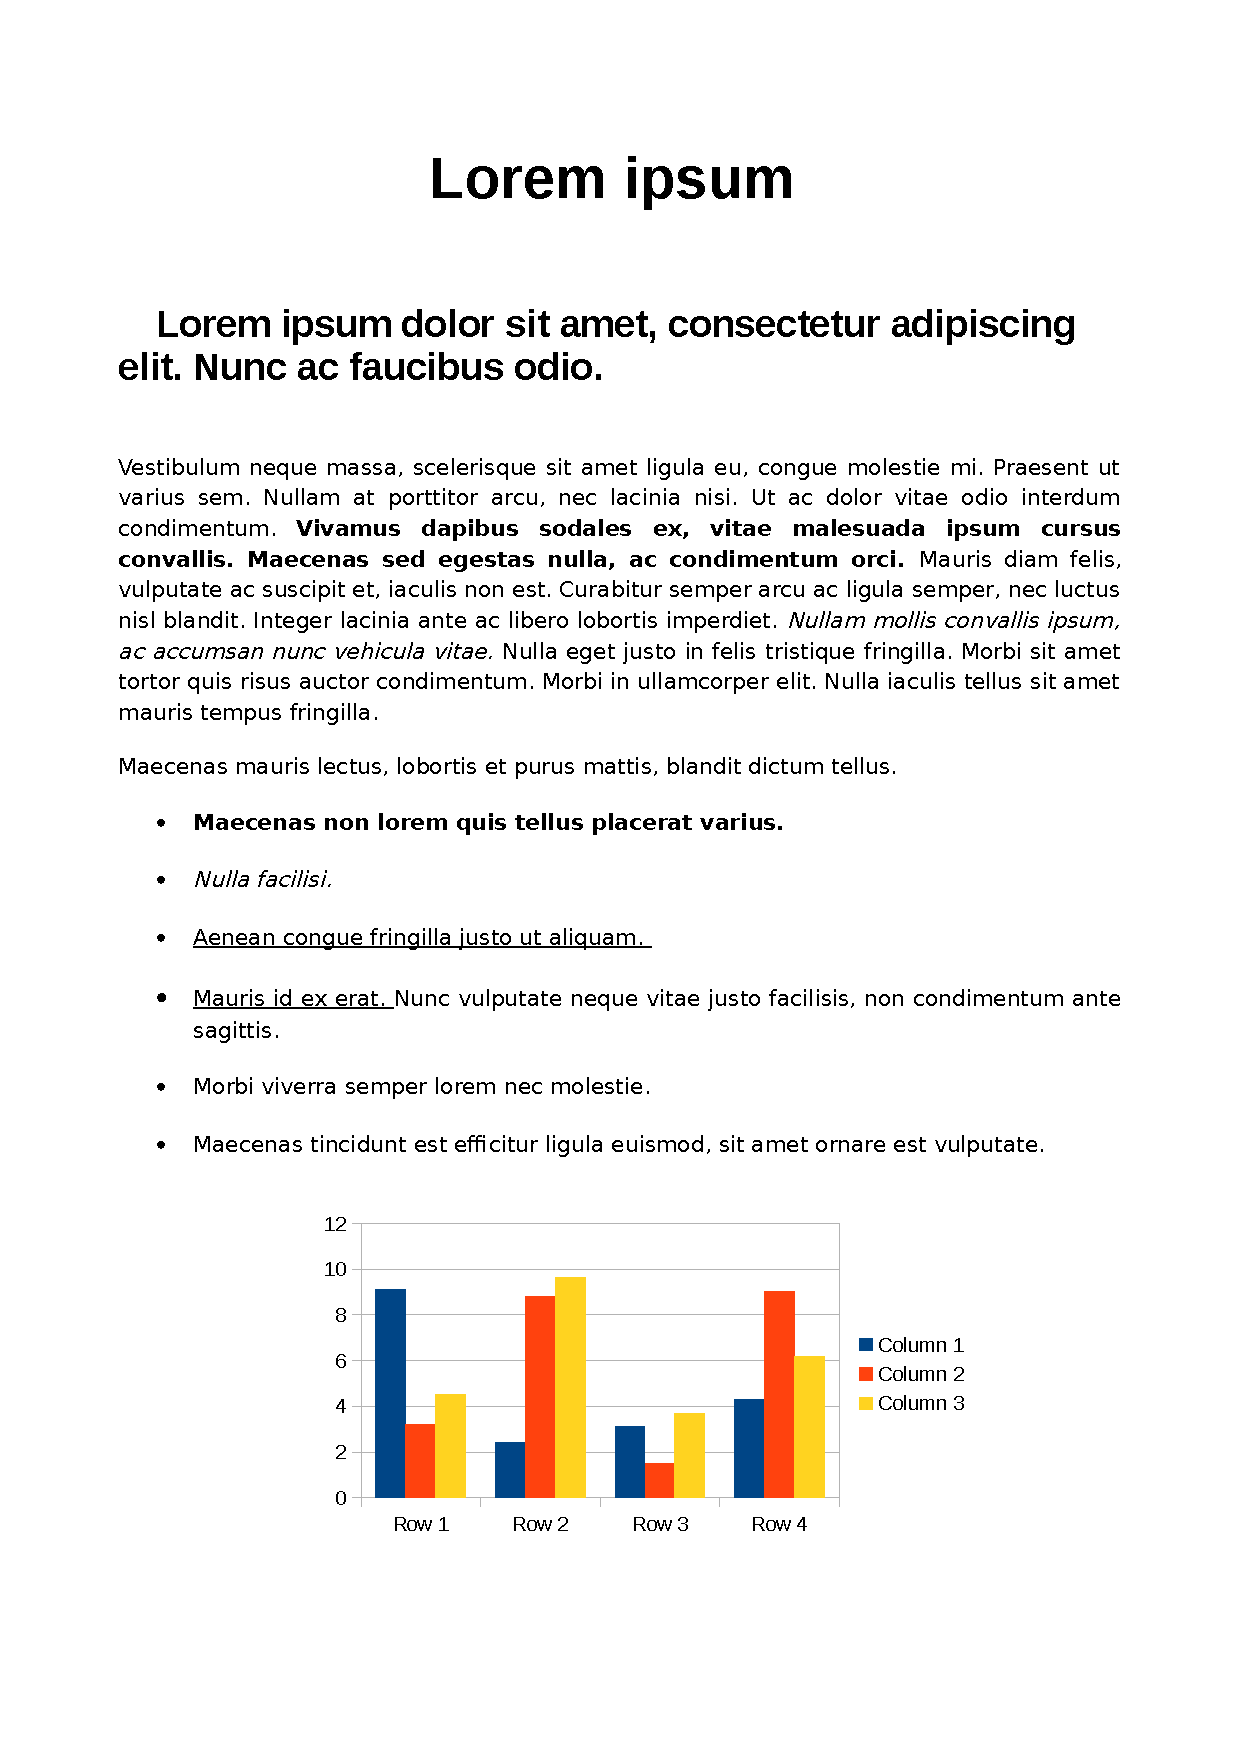
\includepdf[pages={1-}, scale=0.9]{res/documents/file-sample.pdf} % #appendix
%!TEX root = ../thesis.tex

%-----------------------------------------------------------------------------%
% MATHEMATICS
%-----------------------------------------------------------------------------%
%
% This module provides some packages for mathematical stuff like equations,
% matrices, etc.

\usepackage{amsmath}
\usepackage{amssymb} % #mathematics

%-----------------------------------------------------------------------------%
% FIXES
%-----------------------------------------------------------------------------%
% By default this template enables all fixes to improve the compiled result.
% However, if you have any problems or don't want the beheviour, just comment
% out the fix with a `%` sign.
% It is recommended to enable all fixes for the best results.
%!TEX root = ../../thesis.tex

%-----------------------------------------------------------------------------%
% This fix improves the typography and layout of the pdf file.
%-----------------------------------------------------------------------------%

% Fix: Pin chapter headings at top of page.
%\renewcommand*\chapterheadstartvskip{}

% Avoid `Schusterjungen` and `Hurenkinder`
\clubpenalty=10000
\widowpenalty=10000
%!TEX root = ../../thesis.tex

%-----------------------------------------------------------------------------%
% This fix adds support to sans serif fonts.
%-----------------------------------------------------------------------------%

% Load fonts
\usepackage{sourcesanspro}
\usepackage{sourcecodepro}

% Apply sans serif font as default
\renewcommand*{\familydefault}{\sfdefault}

% Set URL to sans serif font
\urlstyle{sf}
%!TEX root = ../../thesis.tex

%-----------------------------------------------------------------------------%
% This fix add a package `scrhack` to supress the deprecation warnings from
% inside the KOMA-scripts.
%-----------------------------------------------------------------------------%

\usepackage{scrhack}
%!TEX root = ../../thesis.tex

%-----------------------------------------------------------------------------%
% This fix uses the microtype package to enable better typography and decrease
% `Overfull` and `Underfull` information output from latex.
%
% If using a bibliography with the biblatex package, the url handling of xurl
% is borken. To solve this issue, load the xurl package after the biblatex
% package.
% https://tex.stackexchange.com/questions/3033/forcing-linebreaks-in-url
%-----------------------------------------------------------------------------%

% Enable better typograhpie to decrease `Overfull` and `Underfull` informations.
\usepackage[activate]{microtype}

% Load this package after `biblatex` to solve url linebreaking in the
% bibliography.
\usepackage{xurl}
%!TEX root = ../../thesis.tex

%-----------------------------------------------------------------------------%
% This fix provides internationalization for listings.
%-----------------------------------------------------------------------------%

\renewcommand{\lstlistingname}{\sListingPhrase}
\renewcommand{\lstlistlistingname}{\sListListingPhrase}

% Do not comment out this fixes, otherwise some other pieces would not work.
%!TEX root = ../../thesis.tex

%-----------------------------------------------------------------------------%
% Support multiple authors for thesis.
% Separate authors by a colon.
%-----------------------------------------------------------------------------%

% Check if multiple authors are included.
\newboolean{multipleAuthors}%
\IfCharInString{,}{\documentAuthor}{%
    \setboolean{multipleAuthors}{true}%
}{%
    \setboolean{multipleAuthors}{false}%
}%
%!TEX root = ../../thesis.tex

%-----------------------------------------------------------------------------%
% Add a new command \source to add sources to figures.
%-----------------------------------------------------------------------------%

% Add source to figures.
\newcommand{\source}[1]{%
    \footnotesize{\sSourcePhrase{}: #1}%
}%